% THIS IS SIGPROC-SP.TEX - VERSION 3.1
% WORKS WITH V3.2SP OF ACM_PROC_ARTICLE-SP.CLS
% APRIL 2009
%
% It is an example file showing how to use the 'acm_proc_article-sp.cls' V3.2SP
% LaTeX2e document class file for Conference Proceedings submissions.
% ----------------------------------------------------------------------------------------------------------------
% This .tex file (and associated .cls V3.2SP) *DOES NOT* produce:
%       1) The Permission Statement
%       2) The Conference (location) Info information
%       3) The Copyright Line with ACM data
%       4) Page numbering
% ---------------------------------------------------------------------------------------------------------------
% It is an example which *does* use the .bib file (from which the .bbl file
% is produced).
% REMEMBER HOWEVER: After having produced the .bbl file,
% and prior to final submission,
% you need to 'insert'  your .bbl file into your source .tex file so as to provide
% ONE 'self-contained' source file.
%
% Questions regarding SIGS should be sent to
% Adrienne Griscti ---> griscti@acm.org
%
% Questions/suggestions regarding the guidelines, .tex and .cls files, etc. to
% Gerald Murray ---> murray@hq.acm.org
%
% For tracking purposes - this is V3.1SP - APRIL 2009

\documentclass{acm_proc_article-sp}

\usepackage{graphicx}
\usepackage{enumitem}
\graphicspath{{./images/}}

\begin{document}

\title{Wireless sensors for detecting rust in caturra coffee: Data structures for the prediction of infected crops.}
%
% You need the command \numberofauthors to handle the 'placement
% and alignment' of the authors beneath the title.
%
% For aesthetic reasons, we recommend 'three authors at a time'
% i.e. three 'name/affiliation blocks' be placed beneath the title.
%
% NOTE: You are NOT restricted in how many 'rows' of
% "name/affiliations" may appear. We just ask that you restrict
% the number of 'columns' to three.
%
% Because of the available 'opening page real-estate'
% we ask you to refrain from putting more than six authors
% (two rows with three columns) beneath the article title.
% More than six makes the first-page appear very cluttered indeed.
%
% Use the \alignauthor commands to handle the names
% and affiliations for an 'aesthetic maximum' of six authors.
% Add names, affiliations, addresses for
% the seventh etc. author(s) as the argument for the
% \additionalauthors command.
% These 'additional authors' will be output/set for you
% without further effort on your part as the last section in
% the body of your article BEFORE References or any Appendices.

\numberofauthors{3} %  in this sample file, there are a *total*
% of EIGHT authors. SIX appear on the 'first-page' (for formatting
% reasons) and the remaining two appear in the \additionalauthors section.
%
\author{
% You can go ahead and credit any number of authors here,
% e.g. one 'row of three' or two rows (consisting of one row of three
% and a second row of one, two or three).
%
% The command \alignauthor (no curly braces needed) should
% precede each author name, affiliation/snail-mail address and
% e-mail address. Additionally, tag each line of
% affiliation/address with \affaddr, and tag the
% e-mail address with \email.
%
% 1st. author
\alignauthor
Juan Pablo Ossa Zapata\\
       \affaddr{Eafit University}\\
       \affaddr{Colombia}\\
       \email{jpossaz@eafit.edu.co}
% 2nd. author
\alignauthor
Mauricio Jaramillo Uparela\\
       \affaddr{Eafit University}\\
       \affaddr{Colombia}\\
       \email{mjaramillu@eafit.edu.co}
\alignauthor
Mauricio Toro\\
        \affaddr{Eafit University}\\
        \affaddr{Colombia}\\
        \email{mtorobe@eafit.edu.co}}
% There's nothing stopping you putting the seventh, eighth, etc.
% author on the opening page (as the 'third row') but we ask,
% for aesthetic reasons that you place these 'additional authors'
% in the \additional authors block, viz.
\date{29 September 2019}
% Just remember to make sure that the TOTAL number of authors
% is the number that will appear on the first page PLUS the
% number that will appear in the \additionalauthors section.

\maketitle
\begin{abstract}
The objective of this project is to analyze and propose a possible solution to the late detection of Roya, one of the most catastrophic plant diseases in history, present in coffee crops in several Latin American countries, including Colombia.  In order to do so, an algorithm implementation is proposed, that through the study of data collected by a network of wireless sensors is able to analyze and predict which crops have or are likely to have this fungus.
The solution to this problem is of paramount importance to the Colombian economy because more than half a million families depend on these crops for their livelihoods.  For this reason, it is our responsibility to contribute to the development of technologies and methods capable of reducing the impact of this infection in the countryside of our country.
\end{abstract}

% A category with the (minimum) three required fields
\category{F.2}{Design and analysis of algorithms}{Data structures design and analysis}

\terms{Coffee Rust, Roya}

\keywords{Pattern matching, Data structures design and analysis} % NOT required for Proceedings

\section{Introduction}
Colombia, a country recognized for its great variety of crops and the quality of its products abroad, has been constantly threatened by the presence of a fungus that has been affecting one of its most internationally desired products: coffee. Composed of more than 563,000 families approximately, the guild of coffee growers makes possible the export of 13.5 million bags of coffee a year, thus achieving coffee to be the main agricultural export product of the country. However, this product has been going through very critical times due to a pest known as Roya which, due to its late diagnosis, is very difficult to treat.
In search of a solution to this problem, a network of wireless sensors was implemented to maintain a set of coffee crops with constant monitoring, where physical and chemical data related to the appearance of this fungus was be collected. The task at hand is therefore to implement efficient algorithms and data structures that allow classification and understanding of the collected data.


\section{Problem}
The problem we face is based on creating, through the use of data structures, a system capable of relating the data already studied of Caturra coffee plants achieving to establish parameters and possible causes that make the Rust appear in coffee crops, so as to know beforehand if there is the presence of this fungus in the studied crop.
To achieve this purpose will represent a great advance for the Colombian agriculture, through its implementation in the cultures of Caturra coffee to diminish the high quantity of cultures lost by cause of the Rust.

\section{Related work}
We present the following related work as the base material for the construction of our own solution to the problem.
\subsection{ID3 algorithm}
ID3 is an algorithm to generate a decision tree created by Ross Quinlan focused on the search for hypotheses or rules based on a set of examples formed by a series of continuous data called attributes in which one will be the attribute to classify. This, also known as objective, is of binary type, that is, it will have values such as positive or negative, yes or no, valid or invalid, etc.
The ID3, based on the previously entered examples, tries to obtain the hypotheses by means of which to classify new instances in positive or negative.

\subsection{C4.5 algorithm}
This algorithm, developed by Ross Quinlan, is an extension of the ID3 algorithm mentioned above. C4.5 constructs decision trees from a set of training data in the same way that ID3 does, using the concept of information entropy. At each tree node, the algorithm chooses a data attribute that divides the set of samples into subsets as efficiently as possible. In this way, the attribute with the highest gain of normalized information is chosen as the decision parameter.

\subsection{CART algorithm}
CART is a technique with which classification and regression trees can be obtained. When the target variable is discrete, classification is used; when it is continuous, regression is used. This algorithm finds the independent variable that best separates our data into groups, expressing it as a rule to assign its corresponding node. Then, for each of the resulting groups, the same process is repeated recursively until it is not possible to obtain a better separation.

\subsection{CHAID algorithm}
CHAID is a classification method for generating decision trees by chi-square statistics to identify optimal divisions. It was proposed by Gordon V. Kass in 1980 and is currently one of the most used in marketing studies.

\section{Design of the data structure}
More than just trying to provide a solution to the main problem itself, we allow one of our goals to be that the implementation of the final algorithm is optimized to allow high volumes of data input. This implies designing a data structure, that the algorithm can use efficiently, such that it takes into consideration the nature of the operations performed.
\subsection{Building blocks of the data structure}
We present the following \textit{'building blocks'} as the set of basic abstract units that allow the representation of the proposed data structure, as well as an explanation of each one of them:
\begin{itemize}
  \item \texttt{DataValue}: A union type that can hold both discrete (as \texttt{int}) and continuous (as \texttt{double}) values.
  \item \texttt{DatasetFeature}: [figure \ref{fig:datasetfeatureblock}] A structure that holds the relevant information required to describe a feature in the dataset, along with the name of that feature.
  \begin{figure}[h]
    \centering
    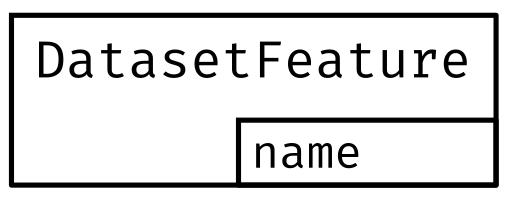
\includegraphics[width=0.14\textwidth]{datasetfeatureblock}
    \caption{Visual representation of the \texttt{DatasetFeature} element.}
    \label{fig:datasetfeatureblock}
  \end{figure}
  \item \texttt{DatasetHeader}: [figure \ref{fig:datasetheaderblock}] A structure that describes the features of the dataset, as well as the label that the algorithm will seek to optimize.
  \begin{figure}[h]
    \centering
    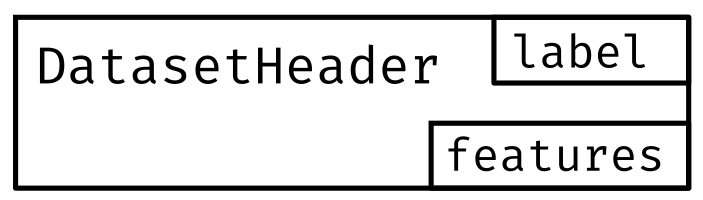
\includegraphics[width=0.17\textwidth]{datasetheaderblock}
    \caption{Visual representation of the \texttt{DatasetHeader} element.}
    \label{fig:datasetheaderblock}
  \end{figure}
  \item \texttt{DatasetEntry}: [figure \ref{fig:datasetentryblock}] A node in the \texttt{Dataset} linked list. It contains an ordered, fixed-size, set of \texttt{DataValue} elements. The size of the set is determined by the number of features in the \texttt{DatasetHeader} of the associated \texttt{Dataset}.
  \begin{figure}[h]
    \centering
    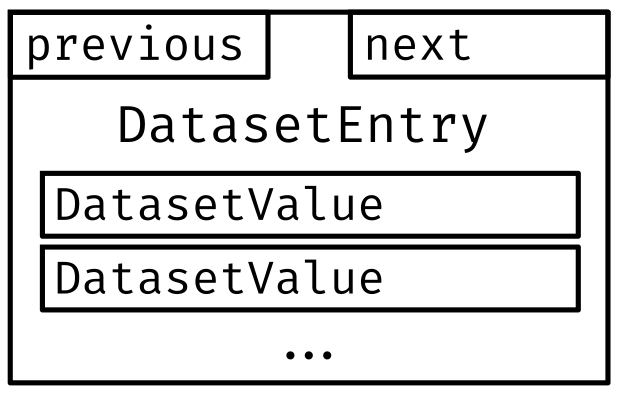
\includegraphics[width=0.17\textwidth]{datasetentryblock}
    \caption{Visual representation of the \texttt{DatasetEntry} element.}
    \label{fig:datasetentryblock}
  \end{figure}
  \item \texttt{Dataset}: [figure \ref{fig:datasetblock}] This is the main substructure. It is essentially a doubly linked list that holds references to the both the head and tail of a chain composed of \texttt{DatasetValue} objects. This structure also has one reference to a \texttt{DatasetHeader}. Some relevant properties arise from the design of this block:
  \begin{itemize}
    \item Fast [$O(1)$] insertion with a reference. This allows loading data from disk with the maximum possible performance.
    \item Full iteration capability. No random access is required, which means that the linked list nature of the structure does not affect the overall performance.
    \item Definition of sub-datasets without increasing the memory usage. As seen in figure \ref{fig:subdataset}, two \texttt{Dataset} objects can have \texttt{head} and \texttt{tail} elements in the same chain, thus allowing the definition of sub-datasets without memory redundancy.
    \begin{figure}[h]
      \centering
      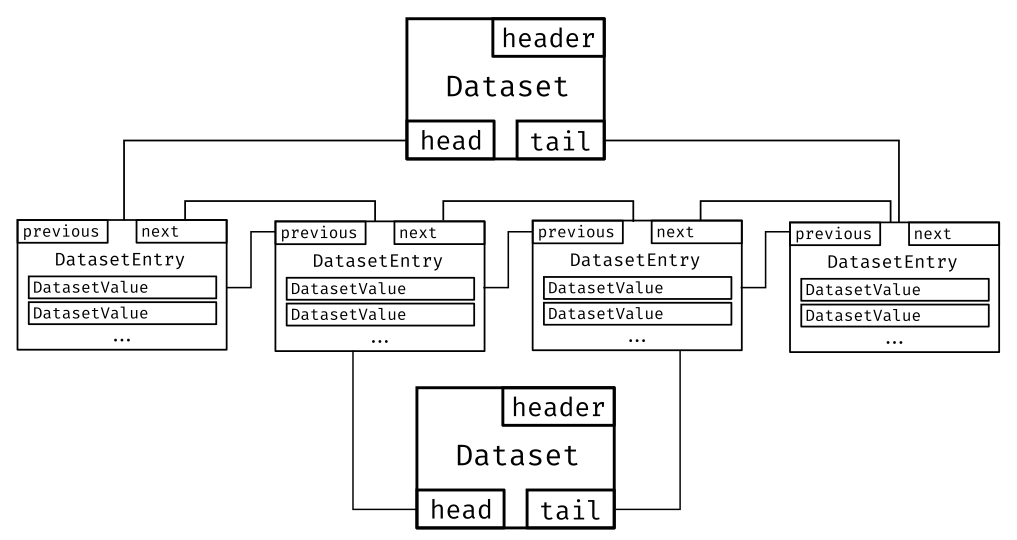
\includegraphics[width=0.5\textwidth]{subdataset}
      \caption{Visual representation of the \textit{sub-dataset} concept.}
      \label{fig:subdataset}
    \end{figure}
  \end{itemize}
  \begin{figure}[h]
    \centering
    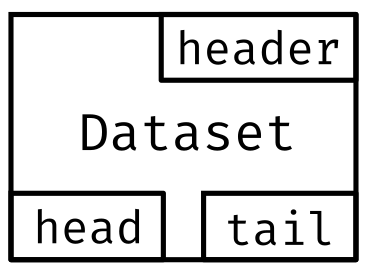
\includegraphics[width=0.10\textwidth]{datasetblock}
    \caption{Visual representation of the \texttt{Dataset} element.}
    \label{fig:datasetblock}
  \end{figure}
\end{itemize}

\subsection{Example data structure usage}
Consider a dataset with the features shown in table \ref{table:1} and the data shown in table \ref{table:2}.
\begin{table}[h]
  \centering
  \begin{tabular}{|c|c|c|}
    \hline
    name                       & type       & label            \\ \hline
    fruit                      & discrete   & yes              \\
    red                        & continuous & no               \\
    green                      & continuous & no               \\
    blue                       & continuous & no               \\ \hline
  \end{tabular}
  \caption{Features of the example dataset.}
  \label{table:1}
\end{table}
\begin{table}[h]
  \centering
  \begin{tabular}{|c|c|c|c|}
    \hline
    fruit                      & red         & green  & blue  \\ \hline
    1 (apple)                      & 246.45      & 10.32  & 1.23  \\
    1 (apple)                      & 235.23      & 30.75  & 3.94  \\
    2 (orange)                     & 217.24      & 184.23 & 11.23 \\
    2 (orange)                     & 250.01      & 120.88 & 0.42  \\ \hline
  \end{tabular}
  \caption{Data of the example dataset.}
  \label{table:2}
\end{table}
Using the proposed data structure, this example dataset would have a similar appearance to that described in figure \ref{fig:examplevisualization}.
\begin{figure}[h]
  \centering
  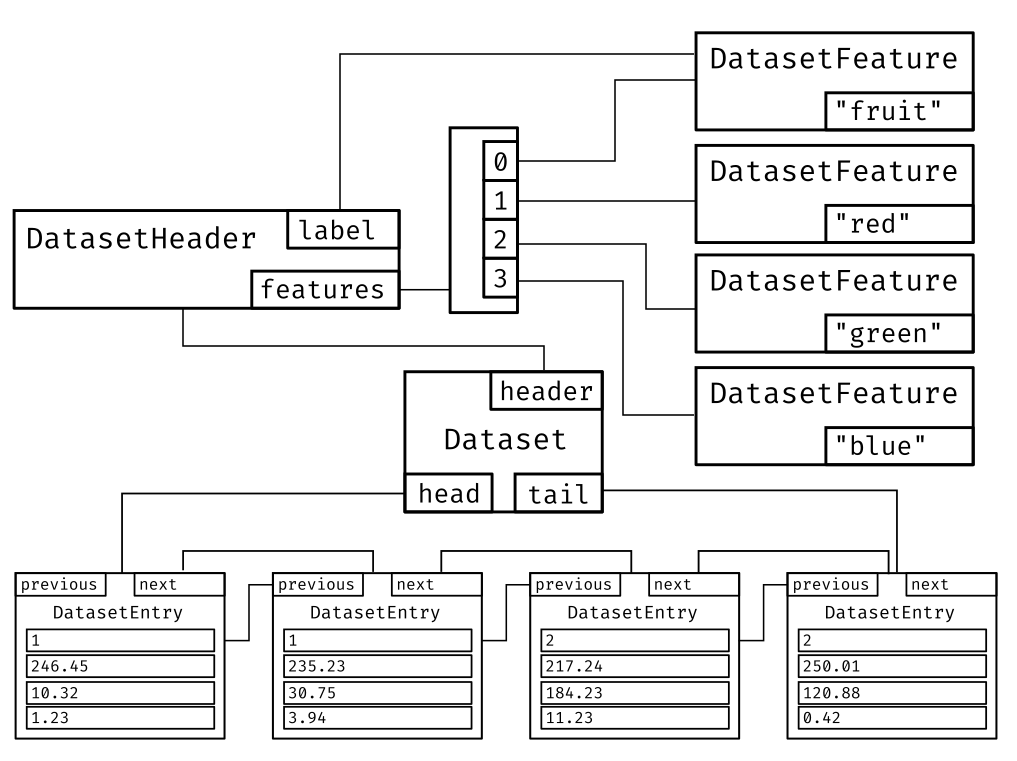
\includegraphics[width=0.5\textwidth]{examplerepresentation}
  \caption{Example dataset appearance.}
  \label{fig:examplevisualization}
\end{figure}
\subsection{Complexity analysis of the data structure}
An analysis of data structure's time complexity provides further information on it's fitness for solving the task. Table \ref{table:3} presents the worst case time complexity for common tasks that the algorithm performs, as well as an explanation on the parameters for said complexity.
\begin{table}[h]
  \centering
  \begin{tabular}{|p{0.10\textwidth}|c|p{0.22\textwidth}|}
    \hline
    Task                             & complexity         & parameters   \\ \hline
    Loading from disk                & $O(n)$      & \begin{itemize}[leftmargin=*]
    \item $n$: The number of entries to be loaded from disk.
    \end{itemize}   \\ \hline
    Find best information gain split & $O(mno)$    & \begin{itemize}[leftmargin=*]
    \item $m$: The number of entries in the dataset.
    \item $n$: The number of features in the dataset.
    \item $o$: Variable proportional to the precision used for split evaluation.
    \end{itemize}   \\ \hline
  \end{tabular}
  \caption{Table of complexity for common tasks.}
  \label{table:3}
\end{table}

\subsection{Data structure benchmarking}
We provide some additional statistics on the exection time and the memory usage of the \texttt{C} implementation of the data structure:
\begin {itemize}
  \item Table \ref{table:4} and figure \ref{fig:loadingtime} show the time used while loading the dataset from disk.
  \begin{table}[h]
    \centering
    \begin{tabular}{|c|c|}
      \hline
      Dataset & time (seconds) \\ \hline
      rust       & 0.00229582 \\
      rust-test  & 0.00109157 \\
      rust-train & 0.00108636 \\ \hline
    \end{tabular}
    \caption{Time used while loading the dataset from disk.}
    \label{table:4}
  \end{table}
  \begin{figure}[h]
    \centering
    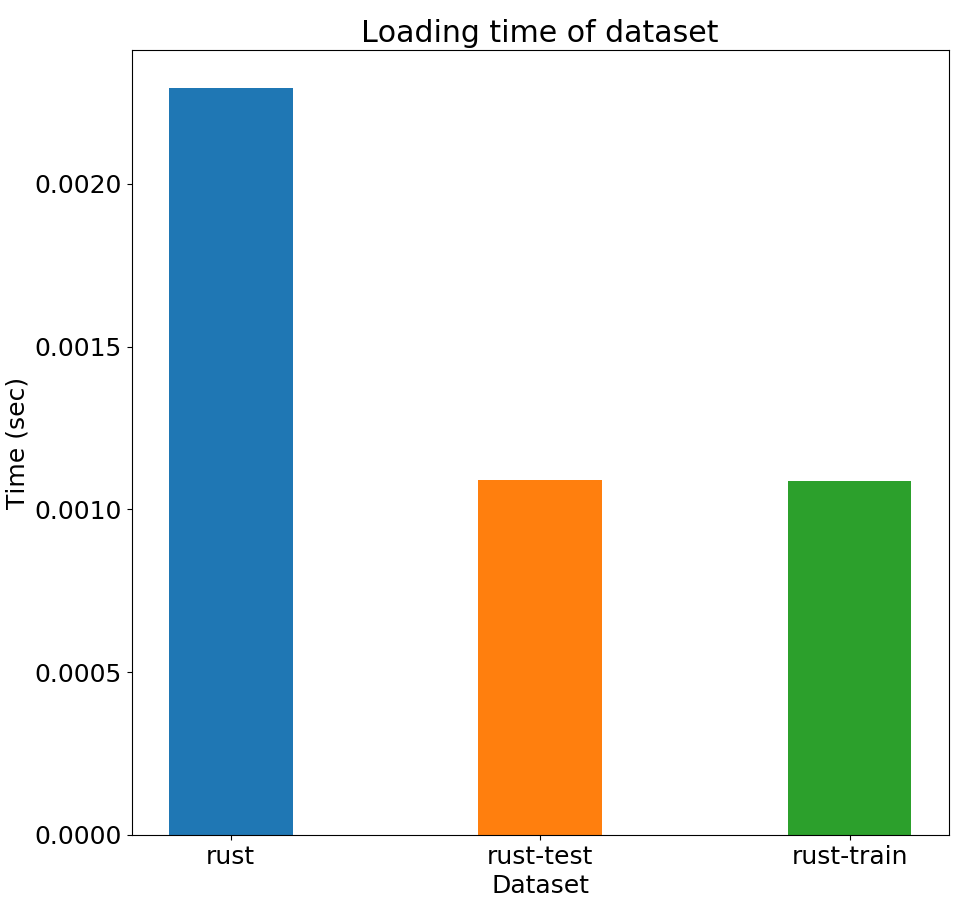
\includegraphics[width=0.4\textwidth]{loadtime}
    \caption{Time used while loading the dataset from disk.}
    \label{fig:loadingtime}
  \end{figure}
  \item Table \ref{table:5} and figure \ref{fig:loadmemoryusage} show the time used while loading the dataset from disk.
  \begin{table}[h]
    \centering
    \begin{tabular}{|c|c|}
      \hline
      Dataset & memory (Kb) \\ \hline
      rust       & 964 \\
      rust-test  & 964 \\
      rust-train & 964 \\ \hline
    \end{tabular}
    \caption{Memory used while loading the dataset from disk.}
    \label{table:5}
  \end{table}
  \begin{figure}[h]
    \centering
    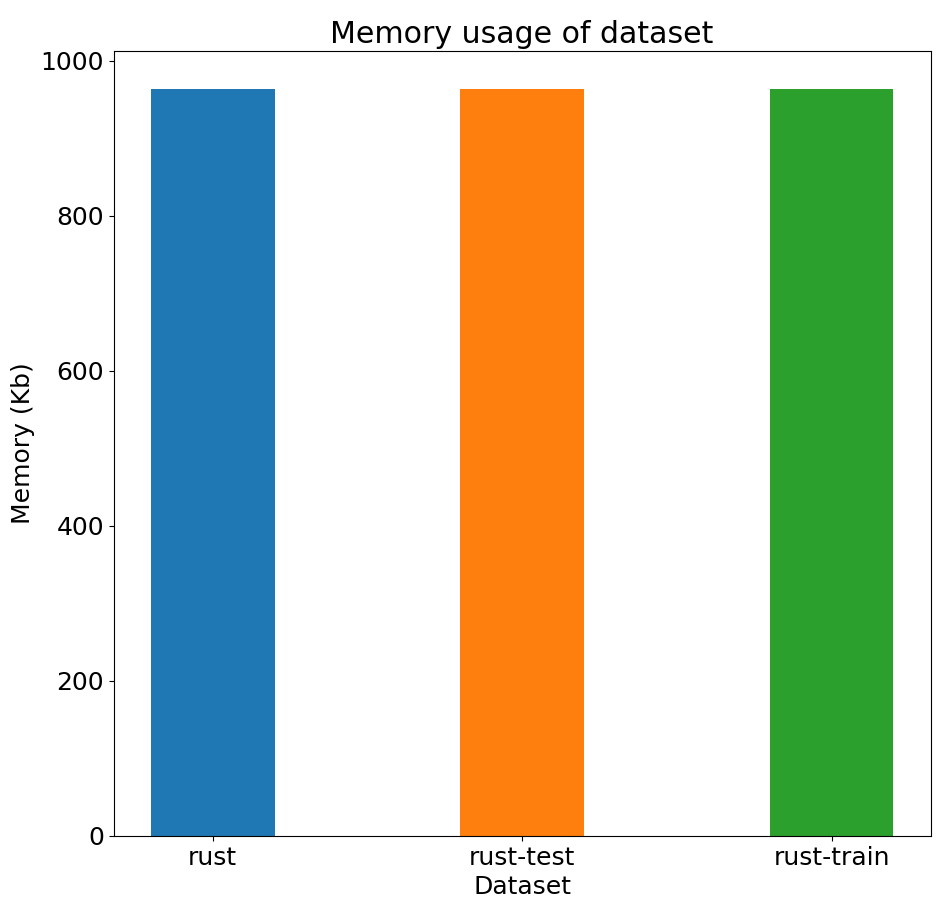
\includegraphics[width=0.4\textwidth]{loadmemoryusage}
    \caption{Memory used while loading the dataset from disk.}
    \label{fig:loadmemoryusage}
  \end{figure}
  \item Table \ref{table:6} and figure \ref{fig:splittime} show the time used while determining a split position that provides the best information gain.
  \begin{table}[h]
    \centering
    \begin{tabular}{|c|c|}
      \hline
      Dataset & time (sec) \\ \hline
      rust       & 3.3113 \\
      rust-test  & 0.2223 \\
      rust-train & 0.2233 \\ \hline
    \end{tabular}
    \caption{Time used while finding split position.}
    \label{table:6}
  \end{table}
  \begin{figure}[h]
    \centering
    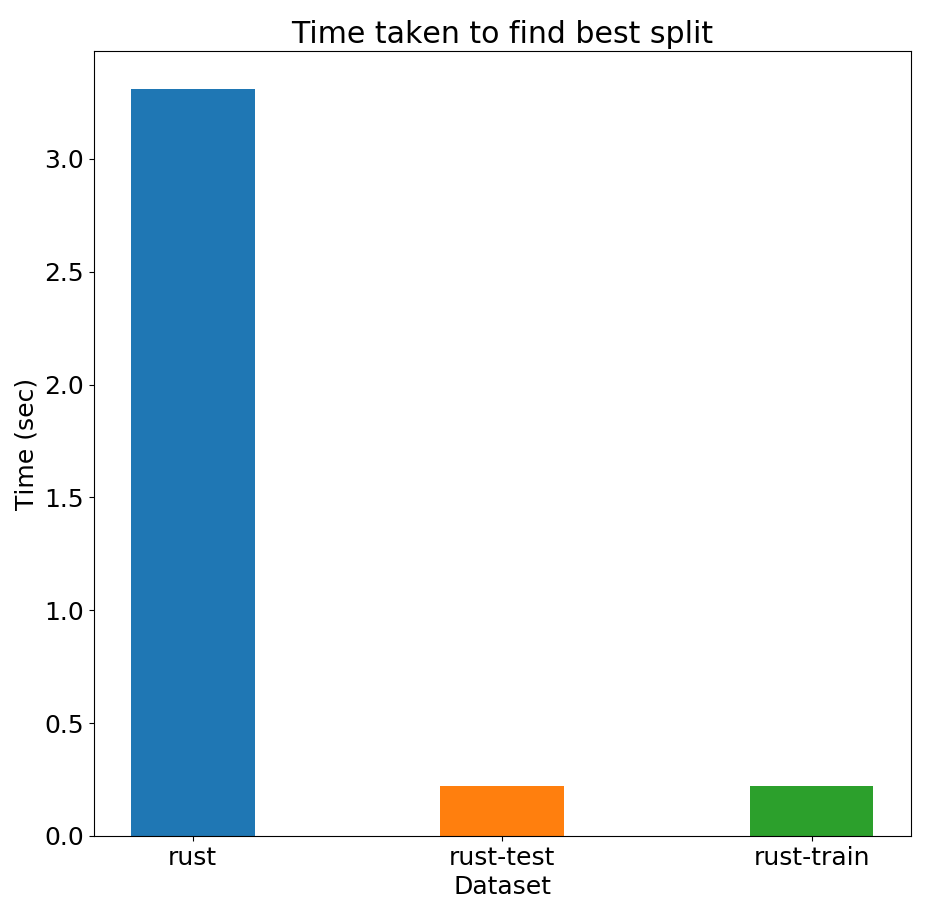
\includegraphics[width=0.4\textwidth]{splittime}
    \caption{Time used while finding split position.}
    \label{fig:splittime}
  \end{figure}
  \item Table \ref{table:7} and figure \ref{fig:splitmemory} show the memory used while determining a split position that provides the best information gain.
  \begin{table}[h]
    \centering
    \begin{tabular}{|c|c|}
      \hline
      Dataset & memory (Kb) \\ \hline
      rust       & 21196.3 \\
      rust-test  & 21196.3 \\
      rust-train & 21196.3 \\ \hline
    \end{tabular}
    \caption{Memory used while finding split position.}
    \label{table:7}
  \end{table}
  \begin{figure}[h]
    \centering
    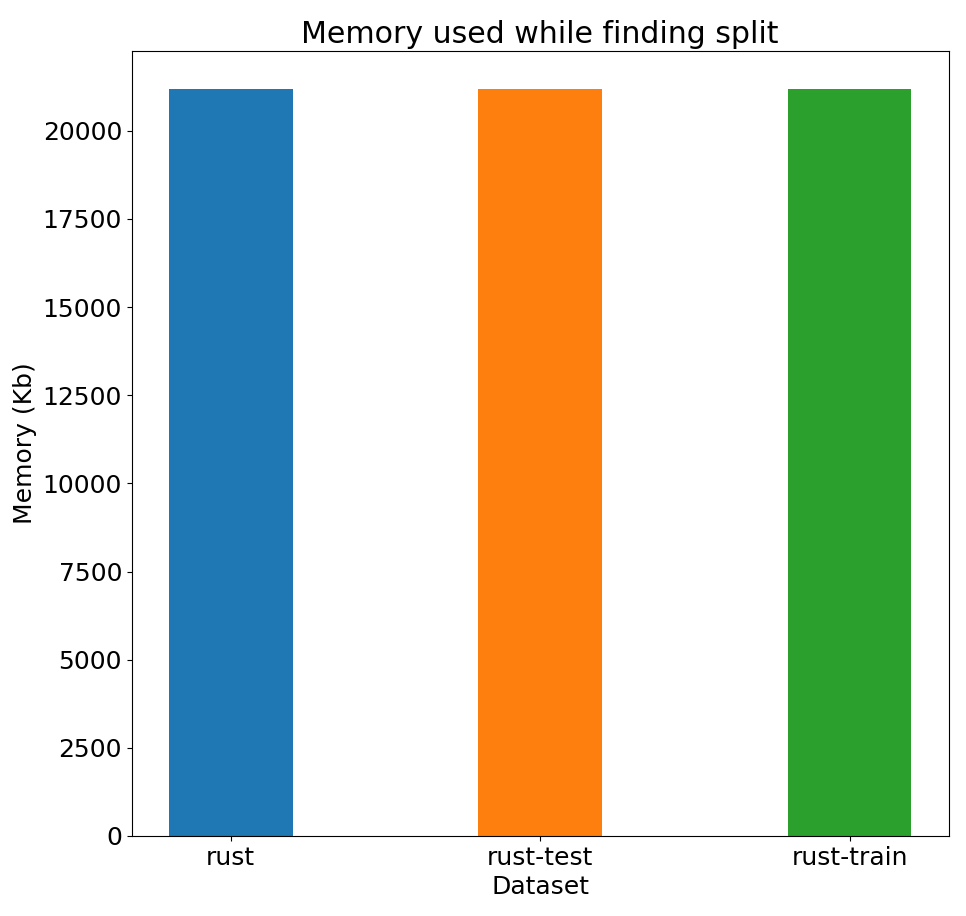
\includegraphics[width=0.4\textwidth]{splitmemory}
    \caption{Memory used while finding split position.}
    \label{fig:splitmemory}
  \end{figure}
\end{itemize}
The fact that the memory usage is the same for all datasets can be explained by the way memory is handled by the program. Unless the difference in sizes of datasets is considerably high, the memory usage will remain the same for all of them.
Also, the reason why the dataset \texttt{rust} takes a longer period of time to find a split position is explained by the fact that the algorithm determined that a higher precision is required for considering a split. This happens because the difference between the upper and the lower boundary of one or more of the features is higher than in the other two datasets. 

\begin{thebibliography}{9}

\bibitem{croplife}
CropLife Latin America. Roya del Cafeto.
\\\texttt{https://www.croplifela.org/es/plagas/listado-de-plagas/roya-del-cafeto}

\bibitem{des_tree}
Charris, L Henríquez, C, Hernández, S, Jimeno, L, Guillen, O, Moreno S.
\textit{Análisis comparativo de algoritmos de árboles de decisión en el procesamiento de datos biológicos}.

\bibitem{ID3}
Centro de Estudios y Aplicaciones Logísticas. Faculty of Engineering of the National University of Cuyo.
\textit{Algoritmo ID3}.

\bibitem{des_r}
Bosco, J.
\textit{Árboles de decisión con R clasificación}.

\bibitem{chaid}
IBM.
\textit{Nodo Chaid}.

\bibitem{cfourfive}
Quinlan, J. R.
\textit{C4.5: Programs for Machine Learning. Morgan Kaufmann Publishers, 1993.}

\end{thebibliography}

\balancecolumns
% That's all folks!
\end{document}
